%!TEX program = lualatex
\documentclass[11pt, a4paper]{scrartcl}
% Packages
\usepackage[margin=1.25in]{geometry}
\usepackage{index}
\usepackage{amsbsy} % Bold math symbols
\makeindex
\usepackage{tcolorbox}
\usepackage{varwidth}
\usepackage{amsmath, amssymb}
\usepackage{esint}
\usepackage{titlesec}
\usepackage{xcolor}
\usepackage{titling}
\usepackage[linktocpage]{hyperref}
\usepackage{pgfplots}
\usepackage{multicol}
\setlength{\columnsep}{2em}
\usepackage{caption}
\usepackage{amsthm}
\usepackage{import}
\usepackage{cancel}
\usepackage{caption}
\usepackage{nicematrix}
\usepackage{mathtools}
\usepackage{enumerate}
\usepackage{graphicx}
\usepackage{tikz}
\usepackage{circuitikz}
\usetikzlibrary{arrows.meta,calc,positioning, angles,quotes}
\usepackage[italian]{babel}
% Font
\usepackage{fontspec}
\setmainfont{Libertinus Serif}

\usepackage{unicode-math}
\setmathfont{Libertinus Math}
% To reset footnote numbering each page
\usepackage[perpage]{footmisc}
\usepackage{setspace}
\setstretch{1.2}

% Titles 
\title{Note di Astrofisica}
\author{Manuel Deodato}
\date{}


% svolgimento
\newenvironment{svolgimento}{\renewcommand\qedsymbol{$\blacksquare$}\begin{proof}[Svolgimento]}{\end{proof}}

\newtheoremstyle{style}% name of the style to be used
{5pt}% measure of space to leave above the theorem. E.g.: 3pt
{5pt}% measure of space to leave below the theorem. E.g.: 3pt
{\normalfont}% name of font to use in the body of the theorem
%{15pt}% measure of space to indent
{0pt}% measure of space to indent
{\noindent\bfseries}% name of head font
{}% punctuation between head and body
{ }% space after theorem head; " " = normal interword space
{\thmname{#1}\thmnumber{ #2}{\thmnote{ (#3)}.\ }}


\theoremstyle{style}
\newtheorem{esempio}{Esempio}[section]
\newtheorem{definizione}{Definizione}[section]
\newtheorem{prop}{Proposizione}[section]
\newtheorem{teorema}{Teorema}[section]
\newtheorem{lemma}{Lemma}[teorema]
\newtheorem{corollario}{Corollario}[teorema]
\newtheorem{osservazione}{Osservazione}[section]
\newtheorem{notazione}{Notazione}[section]

\newtheoremstyle{style1}% name of the style to be used
{5pt}% measure of space to leave above the theorem. E.g.: 3pt
{5pt}% measure of space to leave below the theorem. E.g.: 3pt
{\normalfont}% name of font to use in the body of the theorem
%{15pt}% measure of space to indent
{0pt}% measure of space to indent
{\noindent\bfseries\color{red}}% name of head font
{}% punctuation between head and body
{ }% space after theorem head; " " = normal interword space
{\thmname{#1}\thmnumber{ #2}{\thmnote{ (#3)}.\ }}

\theoremstyle{style1}
\newtheorem{esercizio}{Esercizio}[section]


%% Generic box
\newtcolorbox{eqbox}[1][]
{
colback=gray!10,
arc=0pt,
boxrule=0pt,
title=#1
}

 \newenvironment{boxenv}[1][]{
    \begin{eqbox}[#1]
    }{
   \end{eqbox}
}



%%%%%%%%%% Medie con integrali multipli
\def\Yint#1{\mathchoice
    {\YYint\displaystyle\textstyle{#1}}%
    {\YYint\textstyle\scriptstyle{#1}}%
    {\YYint\scriptstyle\scriptscriptstyle{#1}}%
    {\YYint\scriptscriptstyle\scriptscriptstyle{#1}}%
      \!\iint}
\def\YYint#1#2#3{{\setbox0=\hbox{$#1{#2#3}{\iint}$}
    \vcenter{\hbox{$#2#3$}}\kern-.51\wd0}}
\def\longdash{{-}\mkern-3.5mu{-}} 
   % consider using "\mkern-7.5mu" if esint package is loaded
\def\tiltlongdash{\rotatebox[origin=c]{15}{$\longdash$}}
\def\fiint{\Yint\tiltlongdash}

\def\Zint#1{\mathchoice
    {\YYint\displaystyle\textstyle{#1}}%
    {\YYint\textstyle\scriptstyle{#1}}%
    {\YYint\scriptstyle\scriptscriptstyle{#1}}%
    {\YYint\scriptscriptstyle\scriptscriptstyle{#1}}%
      \!\iiint}
      \def\tilongdash{\mkern6mu{-}\mkern-4mu{-}\mkern-5mu{-}} 
   % consider using "\mkern-7.5mu" if esint package is loaded
\def\titiltlongdash{\rotatebox[origin=c]{15}{$\tilongdash$}}
\def\fiiint{\Zint\titiltlongdash}

%Captions
\captionsetup[figure]{font=footnotesize,labelfont=footnotesize}
\captionsetup[table]{font=footnotesize,labelfont=footnotesize}
%Titlesec
\titleformat{\section}
{\fontsize{15}{20}\sffamily\scshape}
{\normalfont\color{gray}{\fontsize{20}{20}\selectfont\thesection}}
{0.7em}
{}
\hypersetup{colorlinks,breaklinks, linkcolor=[RGB]{74, 122, 164}}
\definecolor{asdf}{HTML}{4a7aa4}
% Personalizza la formattazione della subsection
\titleformat{\subsection}[block]{\fontsize{13}{20}\bfseries}{\normalfont\thesubsection}{.5em}{}


% Personalizza la formattazione della subsubsection
\titleformat{\subsubsection}[block]{\fontsize{12}{20}\bfseries}{\normalfont\thesubsubsection}{.5em}{}

% Maketitle customization
\renewcommand{\maketitle}{
\begin{center}
{\sffamily
{\fontsize{20}{20}\selectfont\MakeUppercase\thetitle}}

\vspace{0.2in}

{\large\scshape\sffamily\theauthor}
\end{center}
}

%Evaluate symbol
\DeclareMathOperator{\di}{d\!}
\newcommand*\Eval[3]{\left.#1\right\rvert_{#2}^{#3}}

%%%%%%% Numero delle equazioni in formato a.b
\numberwithin{equation}{subsection}
%%%%%

%%%%%%%%%% Personalizzazione numeri lista
\renewcommand{\theenumi}{(\arabic{enumi})}

%%%% Table of contents

\usepackage[titles]{tocloft}

\renewcommand{\cftdot}{}
\usepackage{titletoc}
%\setcounter{tocdepth}{2}

%%%%%%%%%%%%%%%% Toc style

% Personalizzazione scritta indice


\begin{document}
\maketitle
\newpage
\tableofcontents 
\newpage
\section{Teoria del trasporto radiativo}
\subsection{Grandezze fondamentali}


Si studia la propagazione delle radiazioni elettromagnetiche dalla sorgente che si desidera osservare fino all'osservatore stesso, trascurando le interazioni microscopiche di tale radiazione con il mezzo che separa sorgente e osservatore, bens\`i concentrandosi sulle sue interazioni a livello macroscopico.
\begin{figure}[!ht]
\centering
\resizebox{1\textwidth}{!}{%
\begin{circuitikz}
\tikzstyle{every node}=[font=\fontsize{14.2pt}{18.5pt}\selectfont]
\draw [ color={rgb,255:red,255; green,175; blue,0}, draw opacity=1 , fill={rgb,255:red,255; green,175; blue,0}, fill opacity=1] (-1.125,16.875) -- (-0.875,16.5) -- (-0.625,16.875) -- (-0.875,17.25) -- cycle;
\node [font=\fontsize{14.2pt}{18.5pt}\selectfont, inner xsep=0.080cm, inner ysep=0.085cm, rounded corners=0.020cm] at (-0.875,16.125) {Sorgente};
\draw  (4.5,18.25) rectangle (12,15);
\draw [-{Stealth[scale=1.5]}, ] (0.375,16.625) -- (3.625,16.625);
\draw [-{Stealth[scale=1.5]}, ] (12.5,16.625) -- (15.875,16.625);
\node [font=\fontsize{14.2pt}{18.5pt}\selectfont, inner xsep=0.080cm, inner ysep=0.085cm, rounded corners=0.020cm] at (17.25,15.125) {Osservatore};
\node [font=\fontsize{14.2pt}{18.5pt}\selectfont, inner xsep=0.080cm, inner ysep=0.085cm, rounded corners=0.020cm] at (8.25,16.625) {Mezzo};
\draw (16.875,17.75) to[short] (17.875,16.75);
\draw (17.875,16.75) to[short] (16.875,15.75);
\draw (17,17.625) to[short] (17,15.875);
\end{circuitikz}
}%
\end{figure}
L'assunzione alla base della trattazione \`e che le scale dimensionali dei mezzi attraversati dalla radiazione siano molto maggiori rispetto alla lunghezza d'onda della radiazione stessa.
In questo limite, la propagazione della radiazione pu\`o essere assunta rettilinea.

Le variabili tramite cui si descrive il campo di radiazione sono $\vec{r}$, $t$ e $\hat{k}$, rispettivamente posizione, tempo e versore d'onda.
L'oggetto che permetter\`a di descrivere il campo della radiazione \`e l'\textit{intensit\`a specifica monocromatica} $I_\nu (\vec{r},t,\hat{k})$.
\begin{center}
	\begin{minipage}
		{.45\columnwidth}
	Si definisce studiando l'energia trasferita dalla radiazione su una superficie infinitesima $dA$, con versore normale $\hat{n}$.
	La quantit\`a di energia trasferita a questa superficie da una radiazione che si muove lungo $\hat{k}$, con frequenza compresa tra $\nu $ e $\nu +d\nu $, entro un angolo solido $d\Omega $ e che si trova in $\vec{r}$ al tempo $t$, \`e data da 
	\[
	dE = I_\nu (\vec{r},t,\hat{k}) \hat{k}\cdot \hat{n} \ dAdtd\Omega d\nu 
	\] 
	\end{minipage}
	\hfill
	\begin{minipage}
		{.45\columnwidth}
	\centering
\resizebox{.6\columnwidth}{!}{%
\begin{circuitikz}
\tikzstyle{every node}=[font=\fontsize{14.2pt}{18.5pt}\selectfont]
\draw [short] (0,13.875) -- (1.25,15.125);
\draw [short] (1.25,15.125) -- (0,16.375);
\draw [short] (0,16.375) -- (-1.25,15.125);
\draw [short] (0,13.875) -- (-1.25,15.125);
\draw [ color={rgb,255:red,255; green,255; blue,255}, draw opacity=1 , fill={rgb,255:red,255; green,255; blue,255}, fill opacity=1] (0,15.125) circle (0.125cm);
\draw [-{Stealth[scale=1.5]}, ] (0,15.125) -- (1.25,16.375);
\draw [-{Stealth[scale=1.5]}, ] (0,15.125) -- (1.25,18.5);
\node [font=\fontsize{14.2pt}{18.5pt}\selectfont, inner xsep=0.080cm, inner ysep=0.085cm, rounded corners=0.005cm] at (-0.125,14.75) {$\vec{r}$};
\node [font=\fontsize{14.2pt}{18.5pt}\selectfont, inner xsep=0.080cm, inner ysep=0.085cm, rounded corners=0.020cm] at (-1.25,16.25) {$dA$};
\node [font=\fontsize{14.2pt}{18.5pt}\selectfont, inner xsep=0.080cm, inner ysep=0.085cm, rounded corners=0.005cm] at (1.5,16.125) {$\hat{n}$};
\node [font=\fontsize{14.2pt}{18.5pt}\selectfont, inner xsep=0.080cm, inner ysep=0.085cm, rounded corners=0.005cm] at (1.5,18.5) {$\hat{k}$};
\draw [ color={rgb,255:red,39; green,123; blue,255}, draw opacity=1 , rotate around={-14:(1.25,18.5)}] (1.25,18.5) ellipse (0.875cm and 0.375cm);
\node [font=\fontsize{14.2pt}{18.5pt}\selectfont, inner xsep=0.080cm, inner ysep=0.085cm, rounded corners=0.020cm] at (2.5,18.375) {$d\Omega$};
\draw [ color={rgb,255:red,39; green,123; blue,255}, draw opacity=1, short] (0,15.125) -- (0.375,18.625);
\draw [ color={rgb,255:red,39; green,123; blue,255}, draw opacity=1, short] (0,15.125) -- (2.125,18.25);
\end{circuitikz}}%
	\end{minipage}
\end{center}
Indicando, poi, con $\theta $ l'angolo tra $\hat{k}$ e $\hat{n}$, si pu\`o scrivere
\begin{equation}
	dE = I_\nu (\vec{r},t,\hat{k}) \cos \theta  \ dAdtd\Omega d\nu 
\end{equation}
Si osserva, quindi, che $I_\nu $ ha le dimensioni di 
\[
\frac{\text{energia}}{\text{superficie }\text{tempo } \text{angolo solido } \text{frequenza}}
\] 
In CGS, allora, le sue unit\`a di misura sono $[I_\nu ] = \mathrm{erg} \, \mathrm{cm} ^{-2} \, \mathrm{s} ^{-1}\, \mathrm{sr} ^{-1} \, \mathrm{Hz} ^{-1}$\footnote{Nell'espressione, $\mathrm{erg} $ \`e l'unit\`a di misura dell'energia e $\mathrm{sr} $ \`e lo steradiante, per la misura adimensionale degli angoli solidi.}.
L'intensit\`a specifica permette di determinare il campo di radiazione, per cui l'intera teoria del trasporto radiativo si basa sul trovare questa quantit\`a.
\marginpar{\textit{Flusso}}
Tramite l'intensit\`a specifica, si possono esprimere il flusso monocromatico $F_\nu $ e il flusso $F$ come
\begin{equation}
F_\nu = \int I_\nu \cos \theta  \ d\Omega  \hspace{1cm} F = \int F_\nu \ d\nu 
\end{equation}
Si nota che, per una radiazione isotropa, $I_\nu $ non dipende da $\hat{k}$, quindi $F_\nu \propto \int \cos \theta d\Omega  = 0$.
\marginpar{\textit{Pressione di radiazione} }
L'impulso trasportato dalla radiazione \`e $dE / c$, direzionato lungo $\hat{k}$; la pressione di radiazione \`e ottenuta come il flusso dell'impulso ortogonale alla superficie su cui incide la radiazione, per cui 
\begin{equation}
P_\nu = \int \frac{dE / c}{dA\, dt}\hat{k}\cdot \hat{n} \ d\Omega = \int \frac{I_\nu }{c} \cos ^2 \theta \ d\Omega 
\end{equation}
Se la radiazione \`e isotropa, allora
\[
P_\nu  = \frac{I_\nu }{c} \int \cos^2 \theta \ d\Omega = \frac{I_\nu }{c} \int _0^{2\pi} d\varphi  \int _0^\pi \cos^2 \theta \sin\theta \ d\theta = \frac{4\pi}{3}\frac{I_\nu }{c}
\] 
\marginpar{\textit{Densit\`a di energia}}
La densit\`a di energia trasmessa dalla radiazione \`e l'energia per unit\`a di volume 
\[
dV = dAds \cos \theta  = dA cdt \cos \theta 
\] 
con $ds = cdt$ tratto percorso in tempo $dt$, quindi 
\begin{equation}
u_\nu  = \int \frac{I_\nu }{c} \ d\Omega \hspace{1cm} u = \int u_\nu  \ d\nu  
\end{equation}
Per radiazione isotropa, si ha
\[
u_\nu  = \frac{4\pi }{c} I_\nu \implies P_\nu  = \frac{u_\nu }{3}
\] 
\marginpar{\textit{Intensit\`a specifica media}}
\`E definita come media rispetto all'angolo solido:
\begin{equation}
J_\nu  = \frac{\int I_\nu  \ d\Omega }{\int d\Omega }= \frac{1}{4\pi} \int I_\nu  \ d\Omega 
\end{equation}
In questo modo, si trova che
\[
u_\nu  = \frac{4\pi}{c} J_\nu 
\] 
\begin{osservazione}
Se la radiazione \`e isotropa, allora $J_\nu  = \frac{I_\nu }{4\pi} \int d\Omega = I_\nu $.
\end{osservazione}
\begin{esempio} [Sfera uniformemente brillante]
\ 

\begin{center}
	\begin{minipage}
		{.6\columnwidth}
		Si vuole calcolare il flusso della radiazione emessa dalla sfera nel punto $P$, a distanza $r$ dal suo centro.
		L'ipotesi di sfera uniformemente brillante corrisponde a una radiazione elettromagnetica emessa di intensit\`a $I = B$ costante, in un qualunque punto interno alla sfera, mentre \`e $0$ altrimenti.
	\end{minipage}
	\hfill
	\begin{minipage}
		{.35\columnwidth}
	\centering
	\begin{tikzpicture}[scale=1.4]
		\draw (0,0) circle (1cm);
		\coordinate (A) at (2,0);
		\coordinate (B) at ({1/2},{-sqrt(3)/2});
		\coordinate (C) at (0,0);
		\draw[dashed] ($(B)!-0.5!(A)$) -- (A);
		\pic[draw, "\scriptsize$\theta_c$", angle eccentricity=1.3, angle radius=0.65cm] {angle=C--A--B};
		\draw (0,0) -- ({1*cos(135)}, {1*sin(135)});
		\node at ({.5*cos(135)+.2}, {.5*sin(135)+.2}) {\footnotesize$R$};
		\draw[dashed] (0,0) -- (2,0) node[above] {\footnotesize$P$};
		\draw[dashed] (0,1.1) -- (1,1.1) node[above] {\footnotesize $r$} -- (2,1.1);
		\draw[dashed] (0,0) -- (B);
		\draw[thick] (2,1.05) -- (2,1.15);
		\draw[thick] (0,1.05) -- (0,1.15);
		\draw[fill] (2,0) circle (1.2pt);
		\draw[fill] (0,0) circle (1.2pt);
	\end{tikzpicture}
	\end{minipage}
\end{center}
Il flusso \`e, allora, determinato da se il segmento che parte da $P$ e lungo $r$ interseca o meno la sfera:
\[
F = \int I \cos \theta  \ d\Omega = 2\pi B \int _0^{\theta _c}  \cos \theta  \sin \theta  \ d\theta  = 2\pi B\frac{1 - \cos^2 \theta _c}{2} = \pi B \sin^2 \theta _c
\] 
Per\`o si sa che $\sin \theta _c = R / r$, quindi $F = \pi B \left(R / r\right) ^2$.
Sulla superficie, $r= R$, quindi $F(R) = \pi B$.
\end{esempio}
\begin{boxenv}[]
\centering Riprendere dalla lezione 2, 50:00.
\end{boxenv}















\newpage
\appendix
\section{Grandezze fondamentali}
In astrofisica, si usa il sistema CGS per le unit\`a di misura, ma grammi e centimetri sono scomodi per le misurazioni degli oggetti di interesse, quindi si utilizzano unit\`a derivate.
\begin{itemize}
	\item Massa solare: $1\, M_{\odot} \approx 2 \times 10^{33}\, \mathrm{g} $.

		Le masse delle stelle si aggirano nell'intervallo $0.08 \div 300 \ M_{\odot} $.
		Per le masse delle galassie, invece, si \`e sull'ordine di $10^{11}\ M_{\odot} $.
		Si stima che siano presenti, nell'universo visibile, un totale di $10^{11}$ galassie.
	\item Distanze.

		Per le distanze, si fa riferimento alla distanza Terra-Sole e si individua $1\, \mathrm{AU}  = 1.5 \times 10^{13}\, \mathrm{cm} $.
Si utilizza il raggio Terra-Sole per calcolare la distanza delle stelle tramite triangolazione.
In particolare, si definisce la parallasse annua come $\pi$ e rappresenta l'angolo che sottende una unit\`a astronomica percorso dalla stella nel corso di mezza rivoluzione della Terra attorno al sole.
\begin{center}
	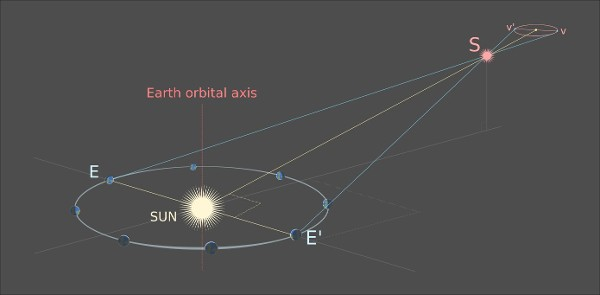
\includegraphics[width=.9\columnwidth]{parallax.jpg}
\end{center}
In questo modo, si ha che 
\[
\tan \pi = \frac{1\, \mathrm{AU} }{d}
\] 
con $d$ distanza tra sole e stella in questione.
Essendo le stelle molto distanti, si considera l'approssimazione $\pi\ll 1$, per cui $\tan \pi \simeq \pi$ e, quindi, $\pi = 1\, \mathrm{AU} / d$.

Visto che gli angoli sono estremamente piccoli, invece di usare i radianti, si fa uso degli arcosecondi.
In questo senso, si definisce una unit\`a di misura per la distanza, il parsec, corrispondente ad una distanza tale che $\pi = 1 \, \mathrm{arcsec} $.
Allora $d[\mathrm{pc} ] = 1[\mathrm{AU} ]/\pi[\mathrm{arcsec}] $.
\item Quanto alle scale temporali, il sole ha $4.57$ miliardi di anni, mentre l'universo ha $13.8$ miliardi di anni.
\end{itemize}
\end{document}
